% Dorien Villafranco
% 08/29/2016
% Reproducing results from "Panel methods for airfoils in turbulent flow" by Glegg, Devenport 2010

\documentclass{article}
\usepackage[letterpaper, margin = 1 in]{geometry}
\usepackage{graphicx}
\graphicspath{.}
\usepackage{float}
\usepackage{caption}
\usepackage{subcaption}


\begin{document}
\noindent \textbf{Establish the Sears Function}\\

\noindent Von Karaman and Sears $(1938)$ analyzed the problem of a thin-airfoil moving through a sinusoidal vertical gust field. The gust was considered as an upwash velocity that is uniformly convected by the free stream. The forcing function was considered to be: 
\begin{equation}
w_g(x,t) = sin\Bigg(w_gt - \frac{w_gx}{V}\Bigg)
\end{equation}
\begin{equation}
w_g(x,t) = sin w_gt cos\Bigg(\frac{w_gx}{V}\Bigg) - cos w_g t sin\Bigg(\frac{w_g x}{V}\Bigg)
\end{equation}

\noindent There were two cases of interested. First, if the gust was referenced to the airfoil's leading edge the equation simply became $w_g(t) = sinw_gt.$ Second, if the gust is referenced to the mid-chord, then x = b = c/2 and the forcing function becomes $w_g(t) cos k_g sin w_gt - sin k_g cos w_g t $which is the equivalent to a phase shift. In the original work of Sears, the mid-chord was used and the lift coefficient was written as: 
\begin{equation}
C_l = 2\pi \Bigg(\frac{w_0}{V}\Bigg)S(k_g)
\end{equation}
where $S(k_g)$ is known as the Sear's function. The gust encounter frequency is given by
\begin{equation}
k_g = \frac{2\pi V}{\lambda_g}
\end{equation}
where $\lambda_g$ is the wavelength of the gust. The figure below outlines the development of the Sear's problem. 
\begin{figure}[h]
\centering
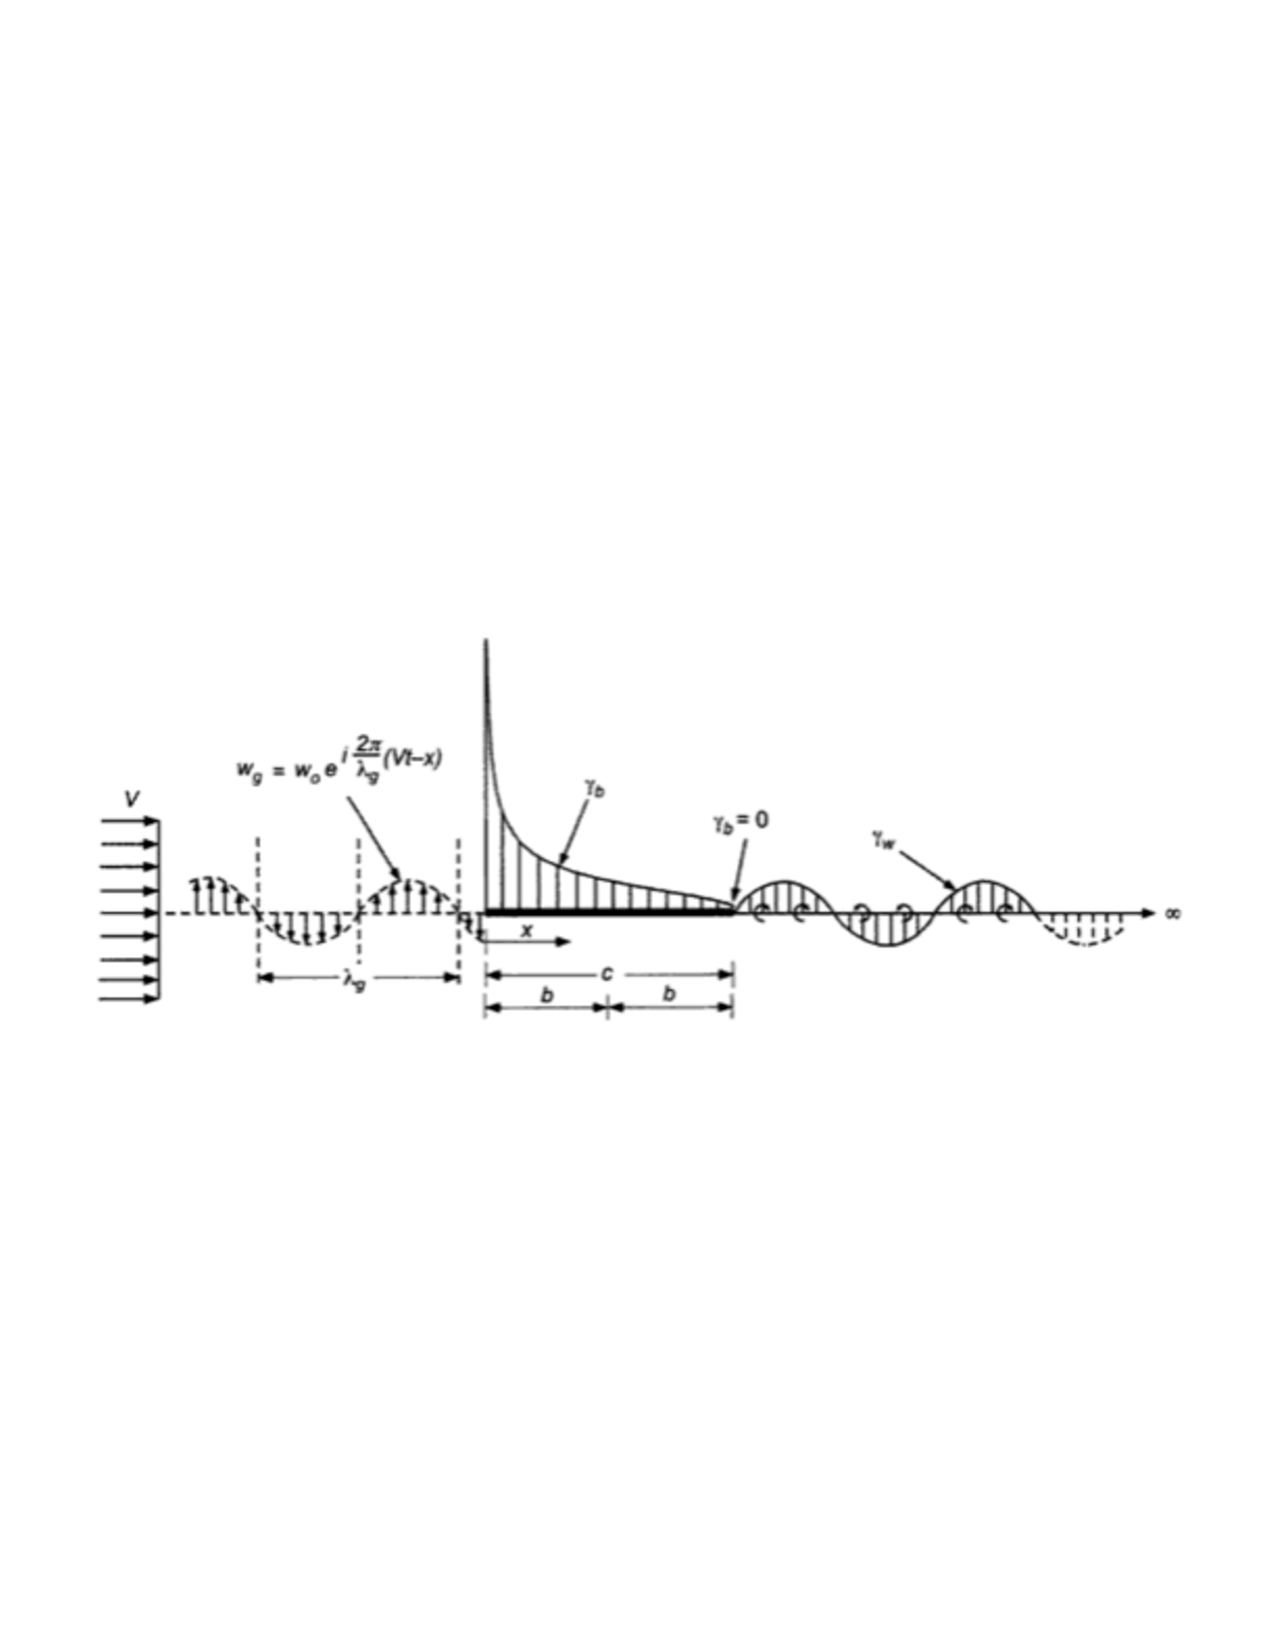
\includegraphics[scale = 0.6]{Sears_Problem}
\caption{Model of thin airfoil encountering a sinusoidal vertical gust (Sear's Problem)}
\end{figure}

\noindent To suit our problem at hand we will redefine the wave number k as: 
\begin{equation}
k = \frac{w c}{2 U}  \qquad  [dimensionless]
\end{equation}
where w is the frequency (2$\pi$f), c/2 is the half chord length and U is the freestream velocity. The Sears function can be expressed in terms of Hankel Functions as shown below: 
\begin{equation}
S(k) = \frac{2}{\pi k (H_{0}^2(k) - i H_{1}^2(k))}  \qquad  [dimensionless]
\end{equation}

\newpage
\noindent From the Sear's function, the analytical lift response of the flat plate to a passing vortex (Blade Vortex Interaction Problem) can be described as:
\begin{equation}
L = \rho \Gamma \frac{c}{2} e^{-kh} \Big(-i S(k) \Big)
\end{equation}

\noindent To match the desired units for Lift as a function of frequency and $x_2$ with k being assumed to being dimensionless, the following equation can be defined: 
\begin{equation}
L(w,x_2) = \rho \Gamma 2R_3 \Big(\frac{c}{2}\Big) e^{-k_1x_2} \Big(-i S(k) \Big) \qquad  \Bigg[\frac{FT}{L}\Bigg]
\end{equation}

\noindent Now if the Lift is made a function of $k_1$ instead of w, 
\begin{equation}
L(k_1,x_2) = \rho U_{\infty} \Gamma 2R_3 \Big(\frac{c}{2}\Big) e^{-k_1x_2} \Big(-i S(k) \Big) \qquad \Bigg[\frac{FL}{L} \Bigg]
\end{equation}
Changing dependency from $x_2$ to $k_2$:
\begin{equation}
L(k_1,k_2) = \frac{1}{2\pi} \int_{-\infty}^{\infty} L(k_1,x_2) e^{-ik_2x_2}dx_2
\end{equation}
Substituting the expression for $L(k_1,x_2)$ into the above equation, the result is:
\begin{equation}
L(k_1,k_2) = \rho \Gamma U_\infty \Big(\frac{c}{2} \Big) \frac{2R_3}{2\pi} \Big(-iS(k_1)\Big) \frac{2k_1}{k_1^2 +k_2^2} \qquad \Bigg[\frac{FL^2}{L}\Bigg]  ??
\end{equation}

The above equation is the blade response per unit span to a harmonic gust. Now that this is defined, it will be used to obtain the unsteady loading spectrum. 
\end{document}